\section{Korisnički profil}

Svaki registrirani korisnik unutar aplikacije ima pregled profila koji služi kao centralno mjesto za pregled svih njegovih penjačkih aktivnosti i analizu napretka. Pristupom profilu korisniku se prikazuje sažetak njegovih penjačkih aktivnosti poput ukupnog broja posjećenih penjališta, ukupan broj zabilježenih uspona te broj dodanih fotografija.

\begin{figure}[H]
    \centering
    \begin{subfigure}[b]{0.3\textwidth}
        \centering
        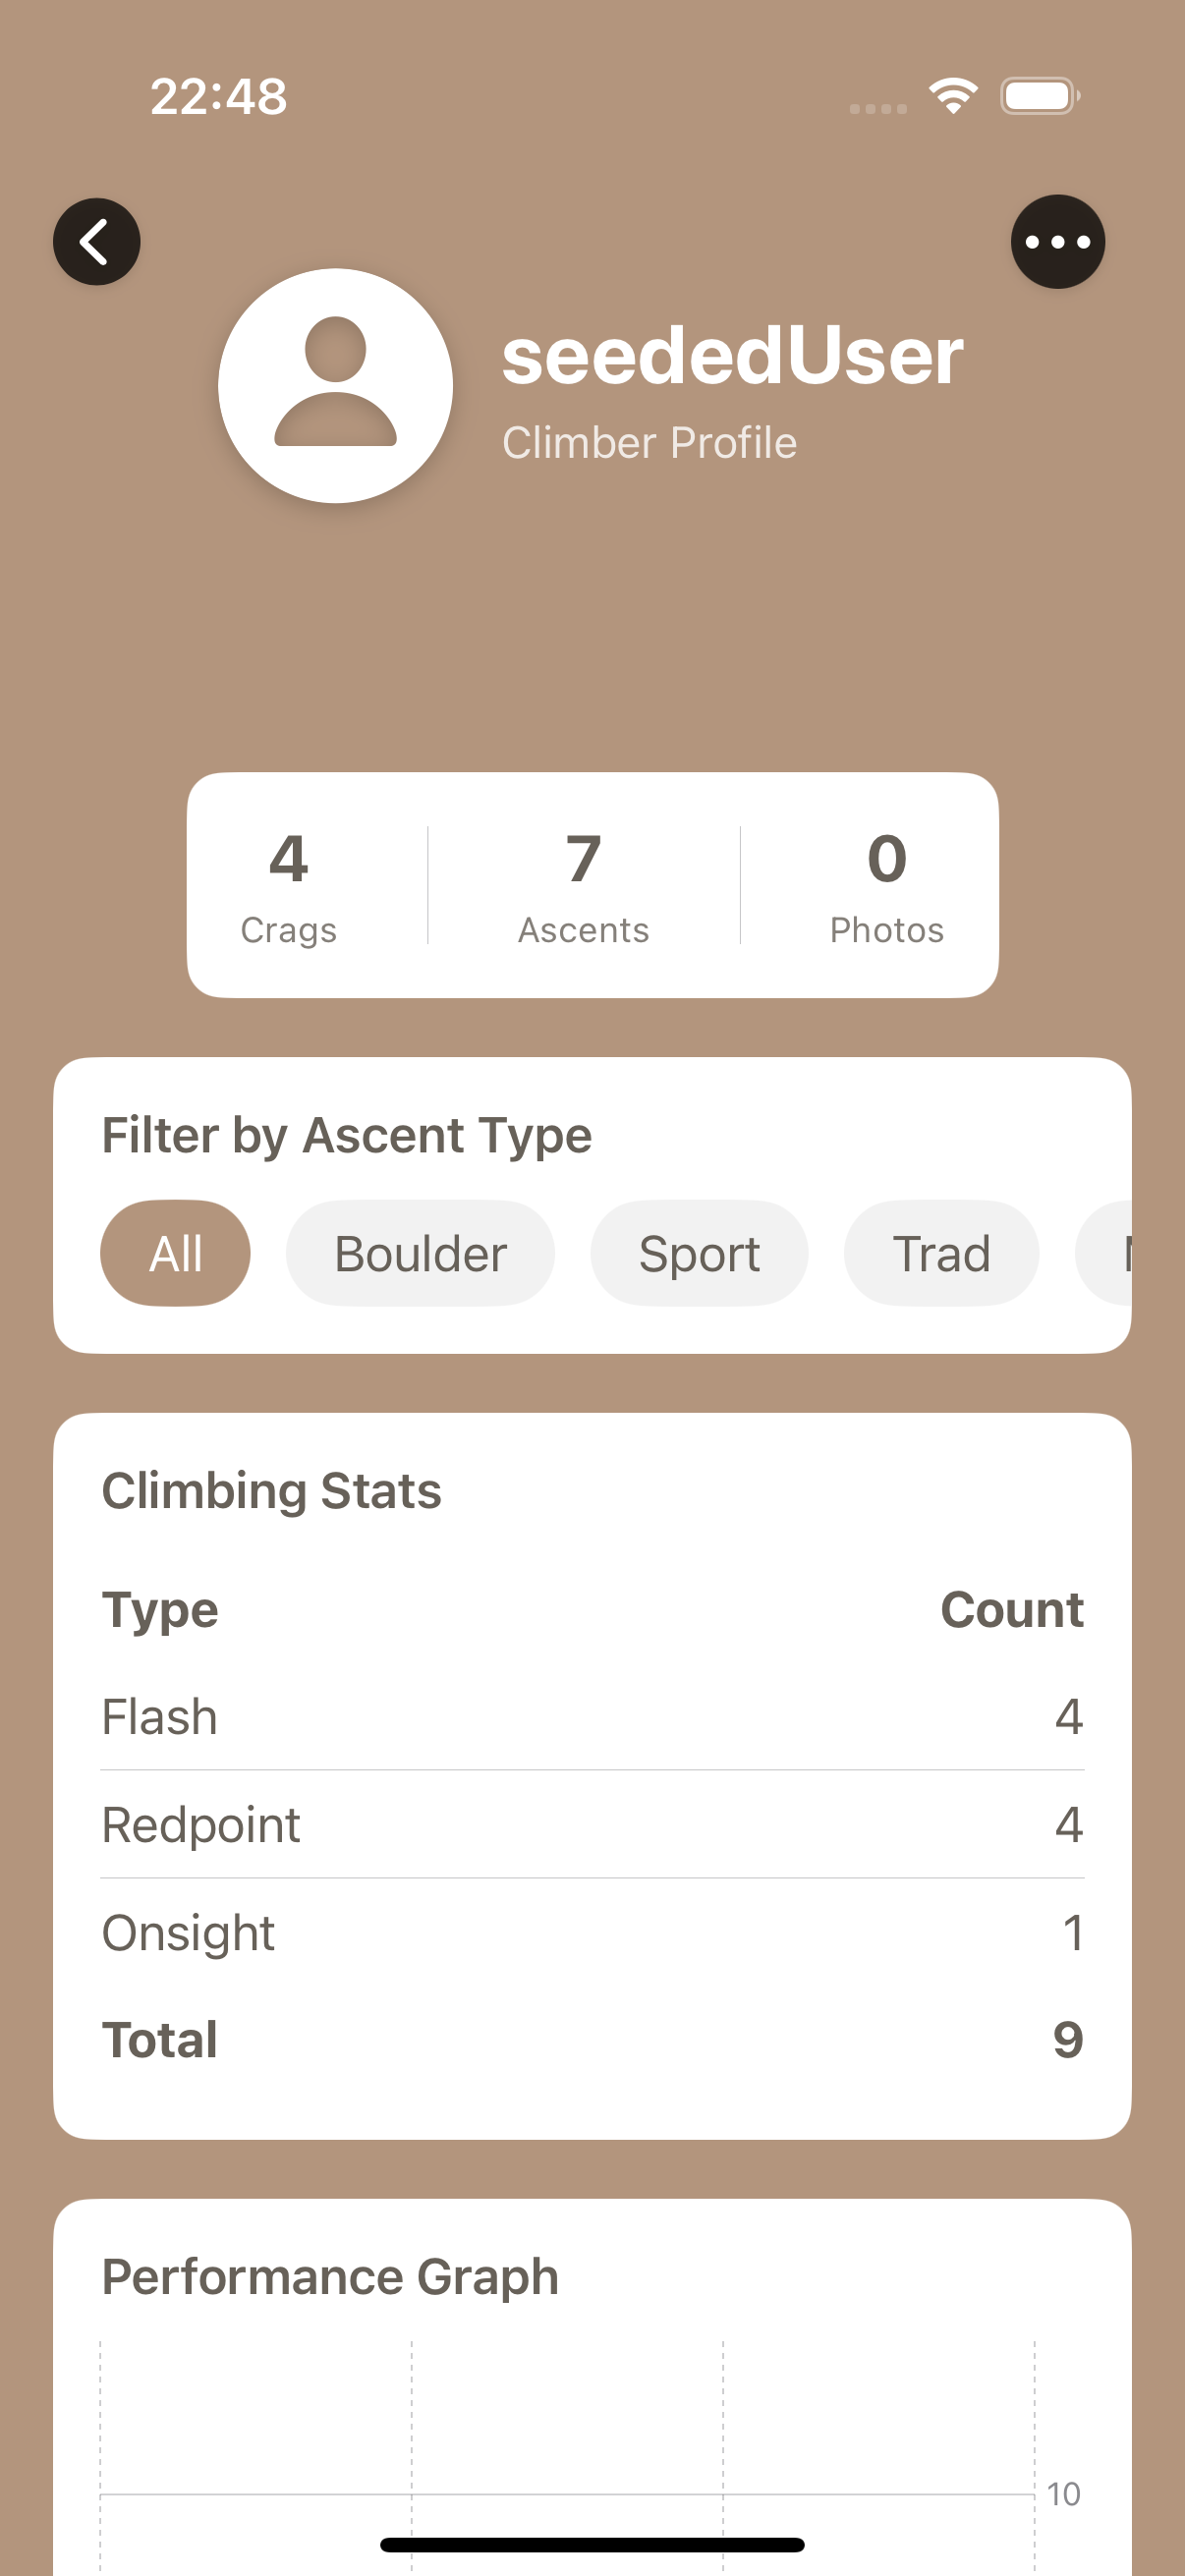
\includegraphics[width=\textwidth]{images/implementacija/user_profile_1.png}
        \caption{Mobilna aplikacija}
        \label{fig:korisnicki_profil_mob}
    \end{subfigure}
    \hfill
    \begin{subfigure}[b]{0.65\textwidth}
        \centering
        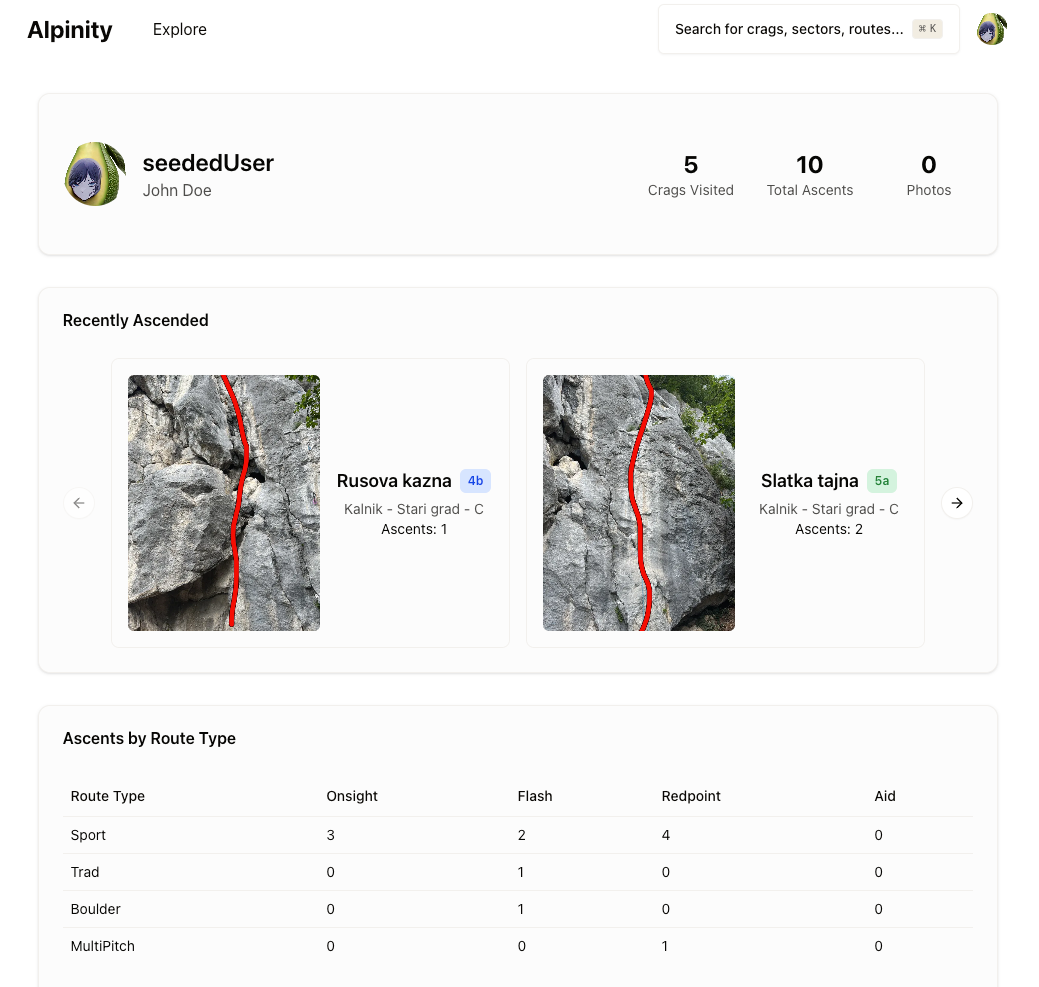
\includegraphics[width=\textwidth]{images/implementacija/web/user-profile-1.png}
        \caption{Web aplikacija}
        \label{fig:korisnicki_profil_web}
    \end{subfigure}
    \caption{Korisnički profil}
    \label{fig:korisnicki_profil}
\end{figure}

Središnji dio profila posvećen je detaljnoj statističkoj analizi (slika~\ref{fig:korisnicki_profil}). Korisnik može filtrirati svoje uspone prema penjačkoj disciplini, poput boulder, sportsko penjanje ili tradicionalno penjanje, kako bi dobio precizniji uvid u svoje aktivnosti. Aplikacija pruža tablični prikaz broja uspona po stilu (Flash, Redpoint, Onsight), omogućujući korisniku da lako vidi koje stilove najčešće prakticira. Dodatno web aplikacija sadrži i nedavno popete penjačke smjerove za korisnika organizirane u horizontalnoj listi sortiranim po datumu uspona od najnovije prema najstarijem.

\begin{figure}[H]
    \centering
    \begin{subfigure}[b]{0.3\textwidth}
        \centering
        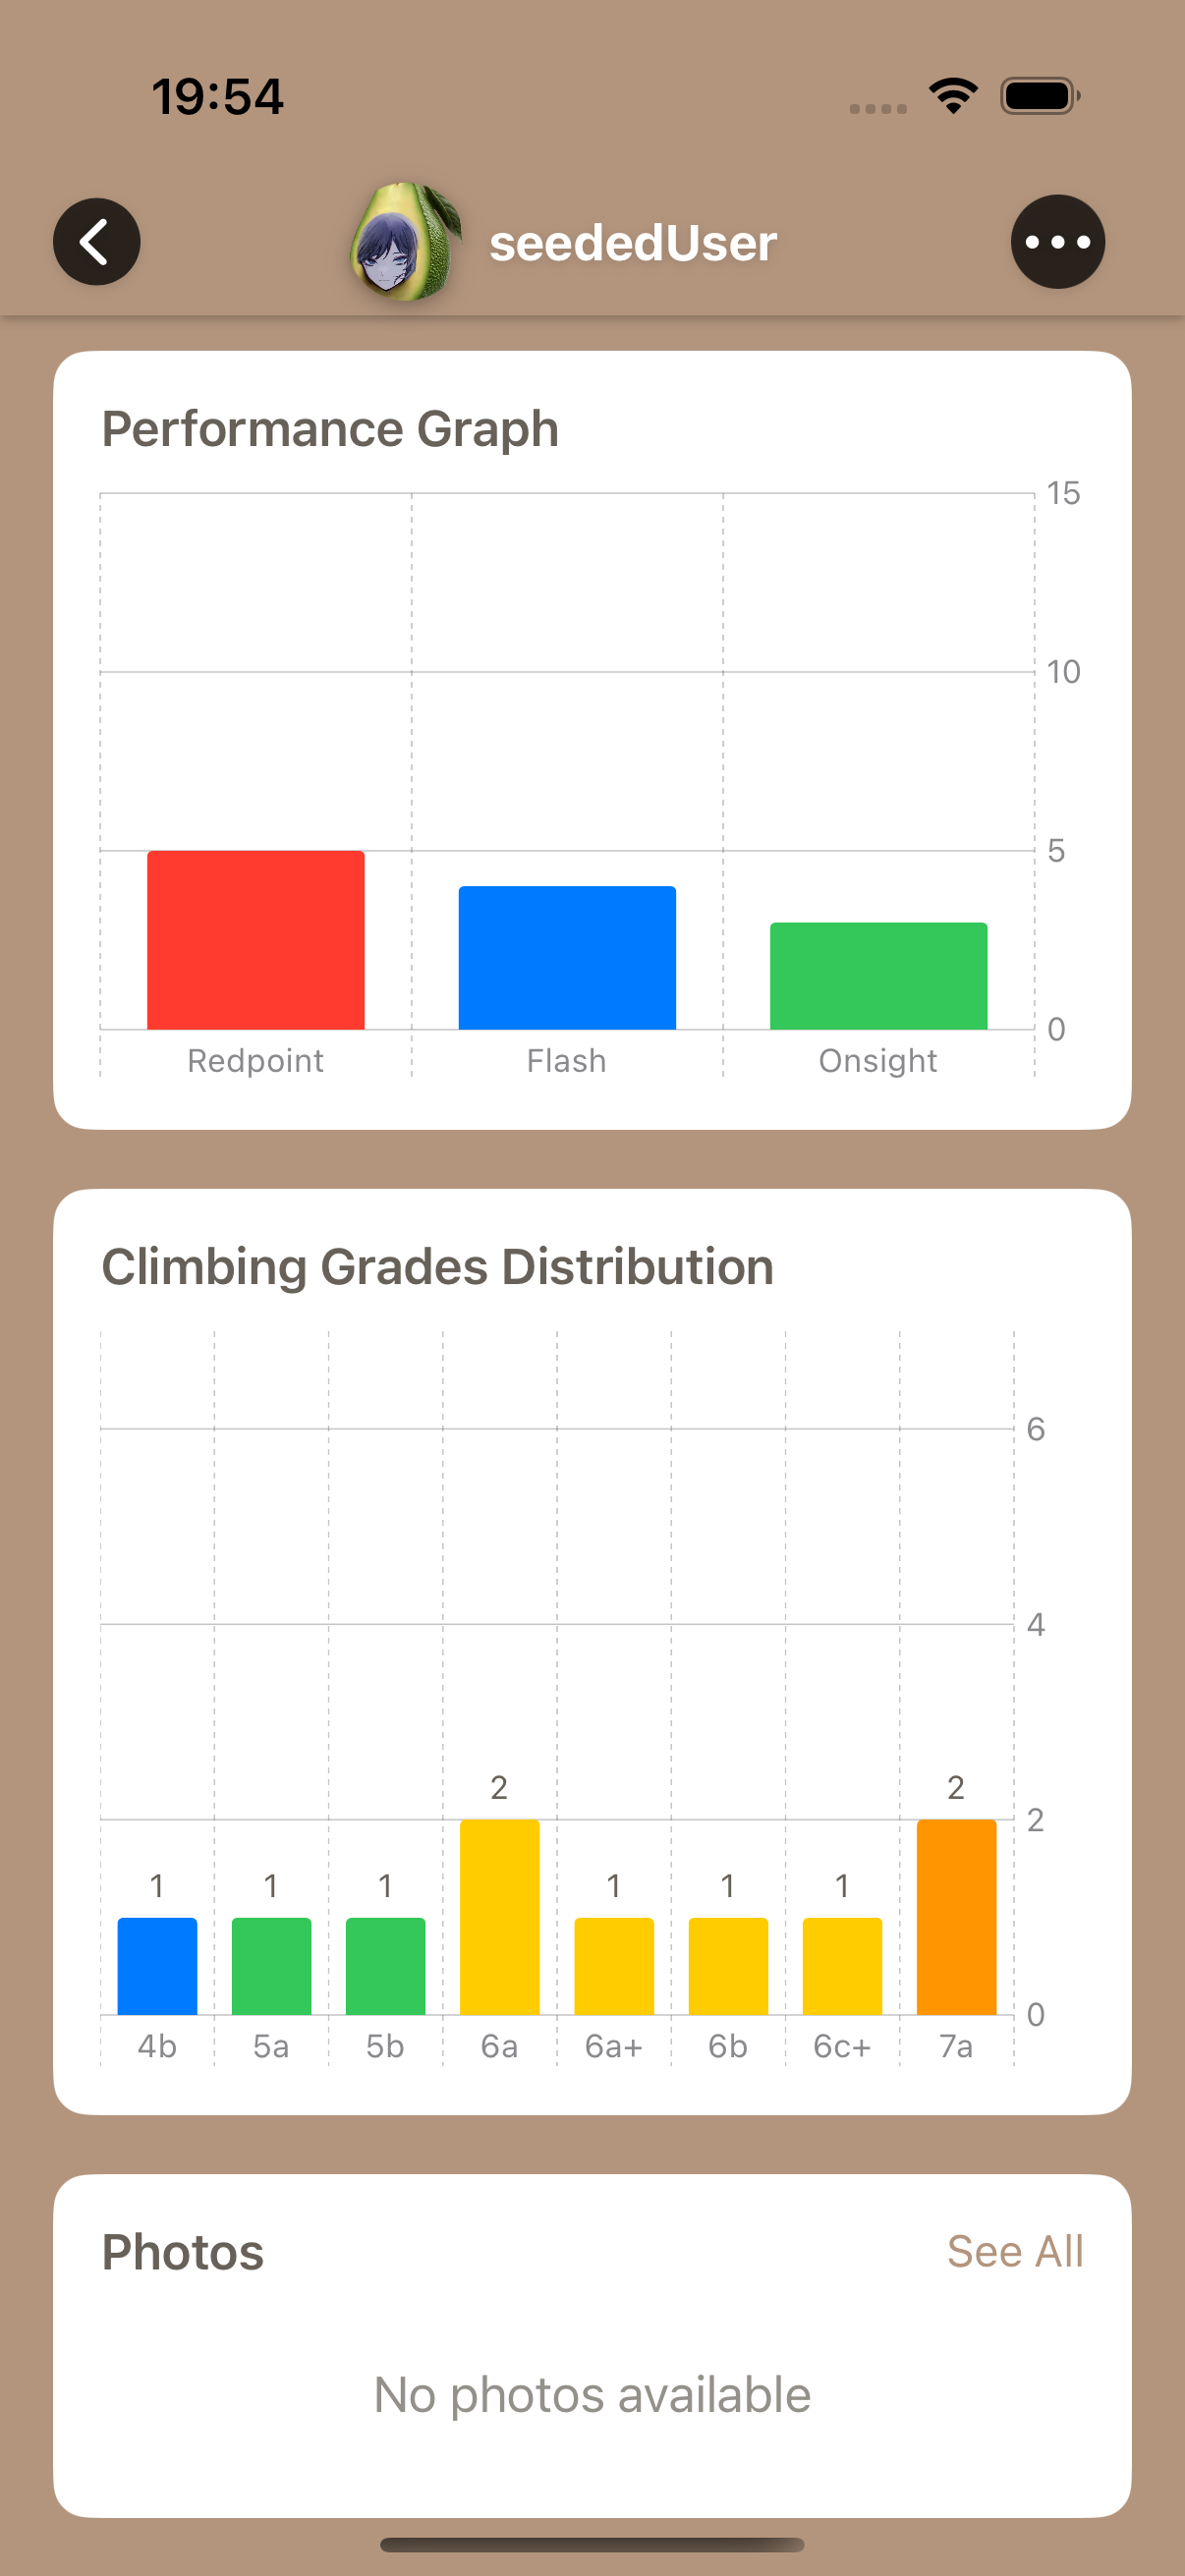
\includegraphics[width=\textwidth]{images/implementacija/user_profile_2.png}
        \caption{Mobilna aplikacija}
        \label{fig:korisnicki_profil_graf_mob}
    \end{subfigure}
    \hfill
    \begin{subfigure}[b]{0.65\textwidth}
        \centering
        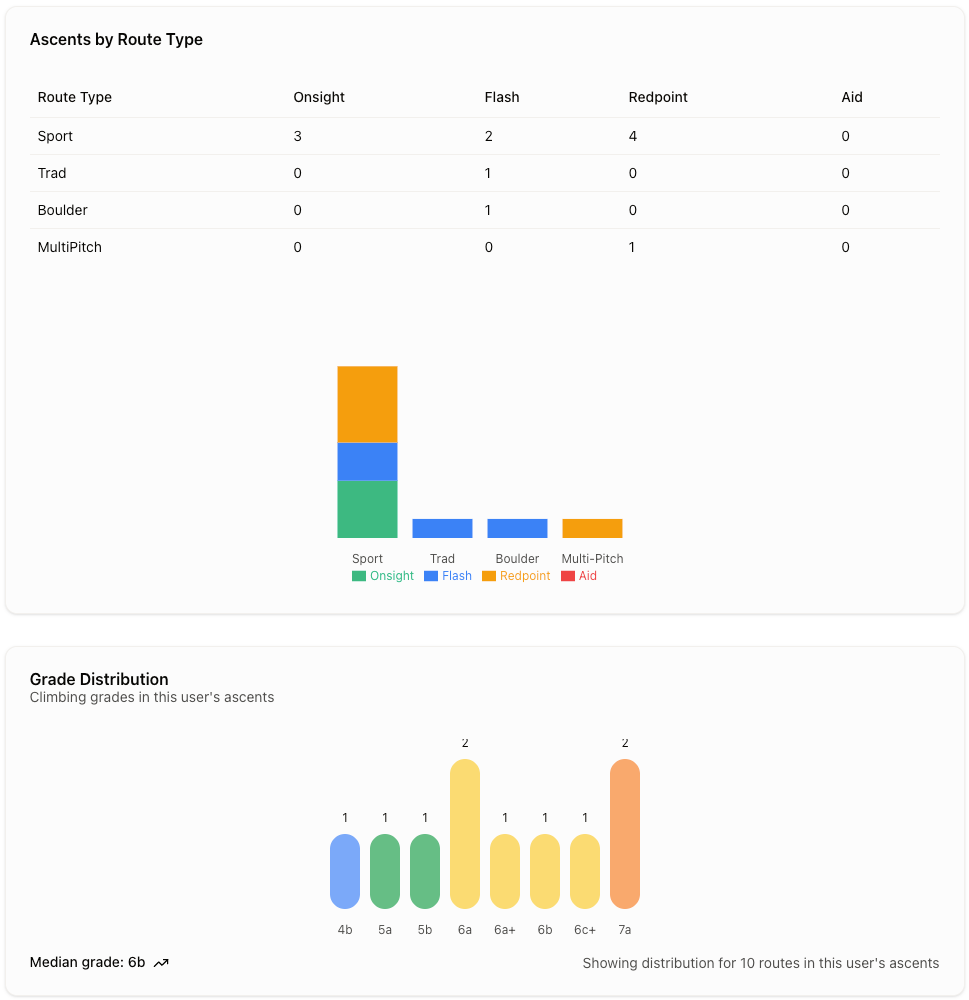
\includegraphics[width=\textwidth]{images/implementacija/web/user-profile-2.png}
        \caption{Web aplikacija}
        \label{fig:korisnicki_profil_graf_web}
    \end{subfigure}
    \caption{Grafovi performansi i distribucije po ocjenama}
    \label{fig:korisnicki_profil_2}
\end{figure}

Za bolju vizualizaciju, podaci su prikazani i u dva ključna grafa (slika~\ref{fig:korisnicki_profil_2}). Graf performansi prikazuje distribuciju uspona po stilu, dok graf distribucije po ocjenama prikazuje stupčastim diagramom, odnosno koliko je penjačkih smjerova određene težine je korisnik uspješno popeo. Ovi grafički prikazi omogućuju procjenu vlastitih sposobnosti i napretka tokom vremena. Finalno na dnu profila nalazi se i lista svih slika kojima korisnik želi istaknuti svoj profil.

\begin{figure}[H]
    \centering
    \begin{subfigure}[b]{0.33\textwidth}
        \centering
        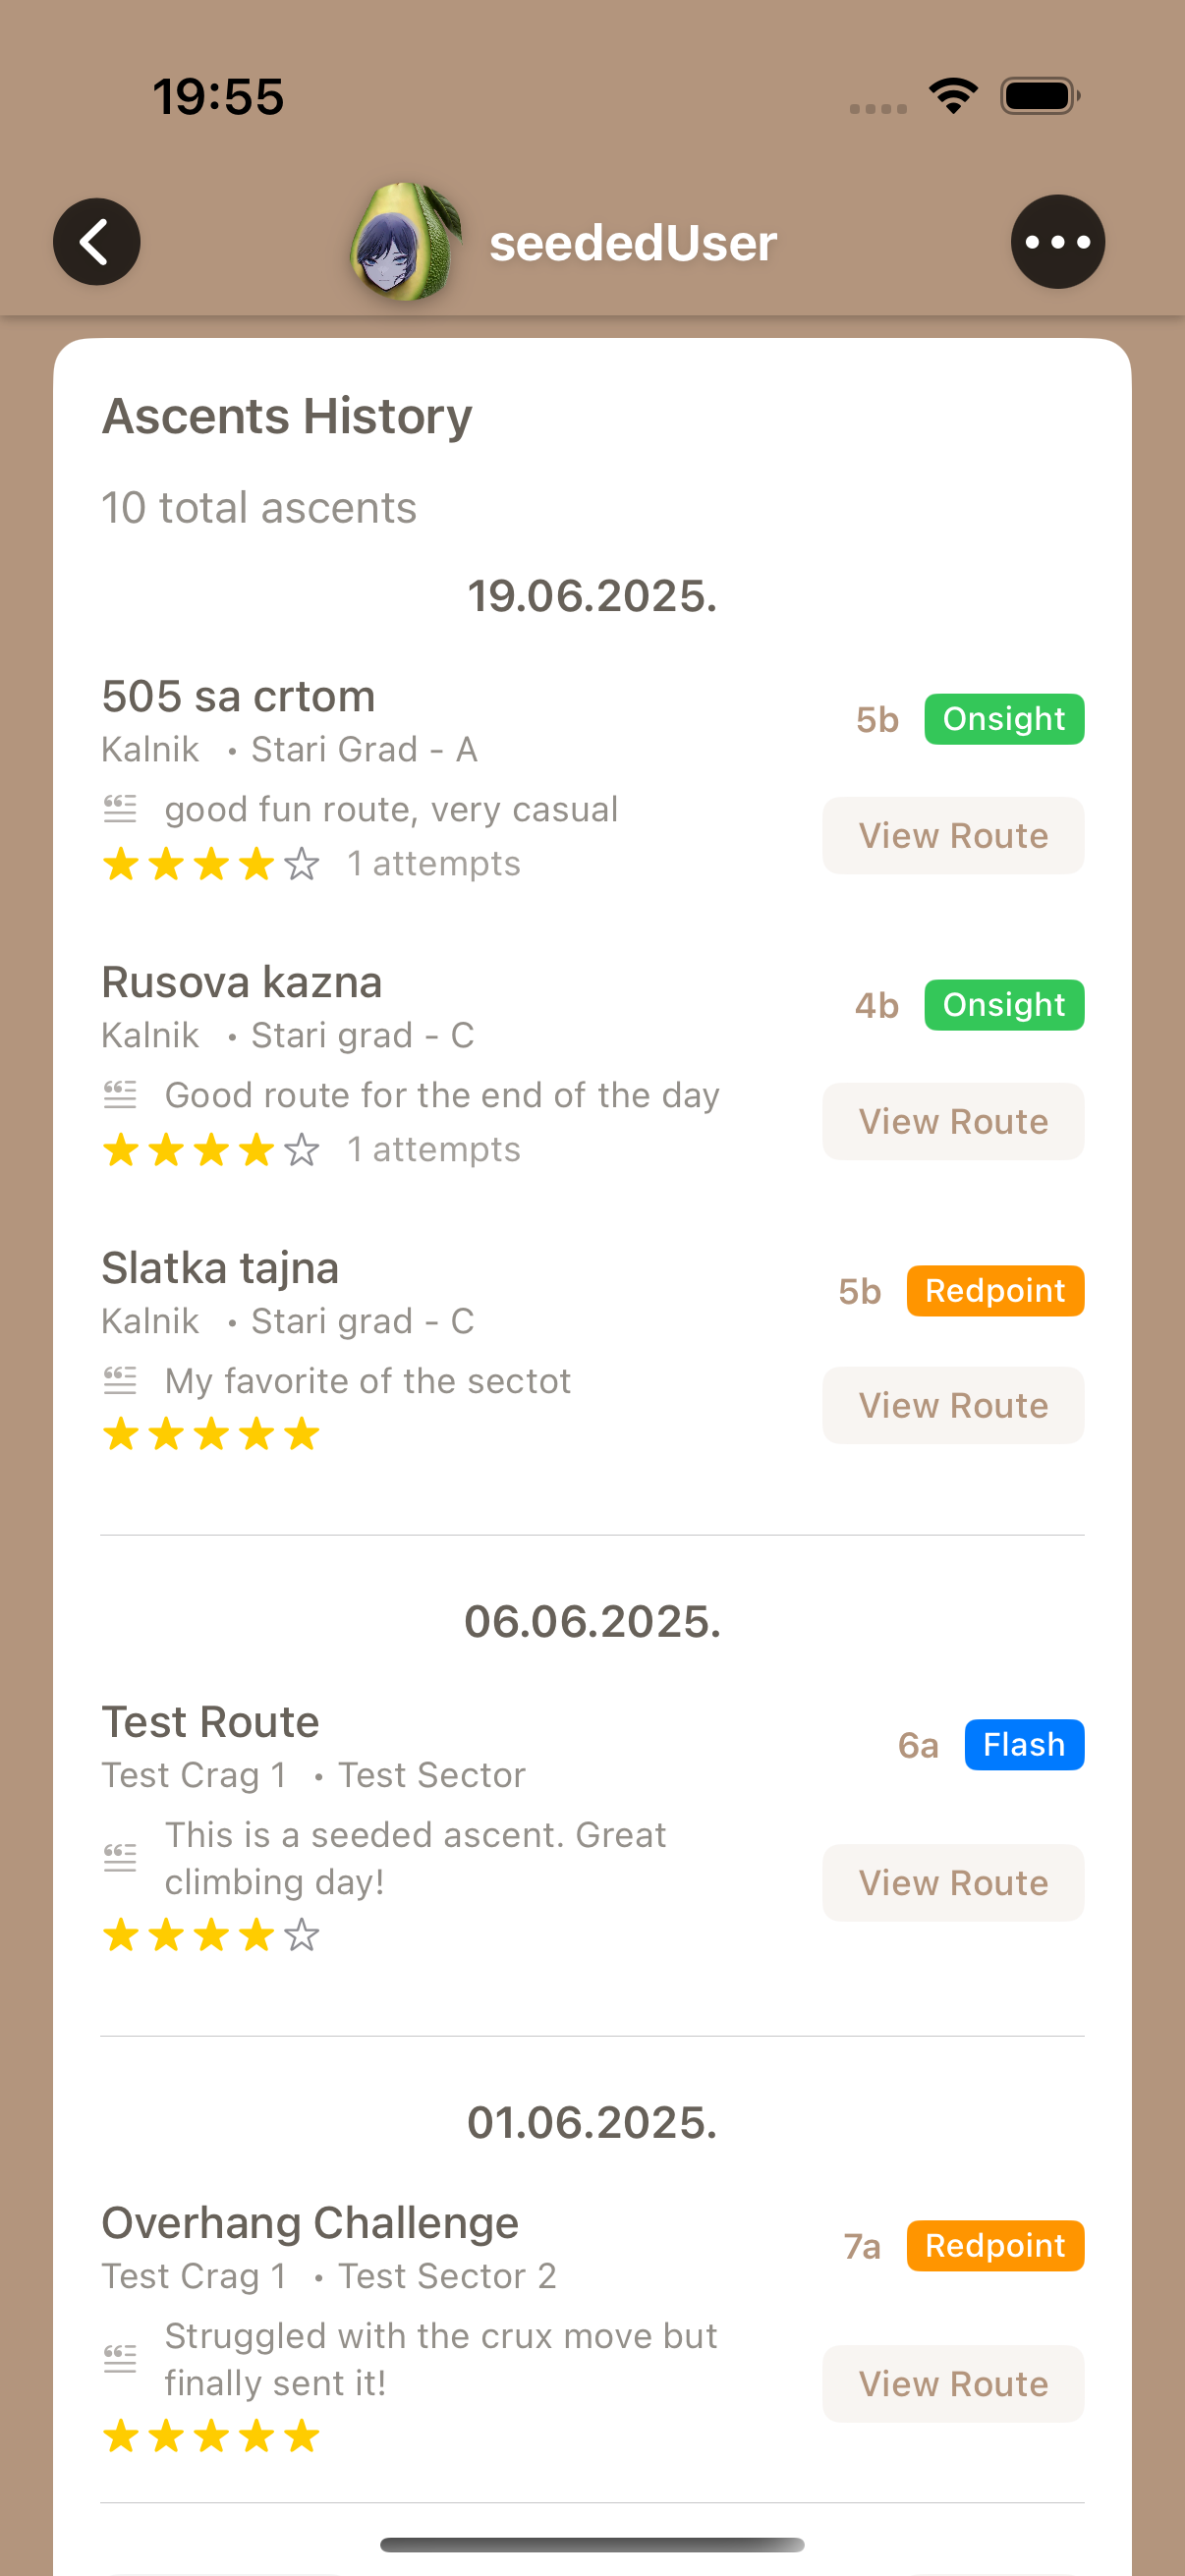
\includegraphics[width=\textwidth]{images/implementacija/user_profile_3.png}
        \caption{Mobilna aplikacija}
        \label{fig:korisnicki_profil_povijest_mob}
    \end{subfigure}
    \hfill
    \begin{subfigure}[b]{0.65\textwidth}
        \centering
        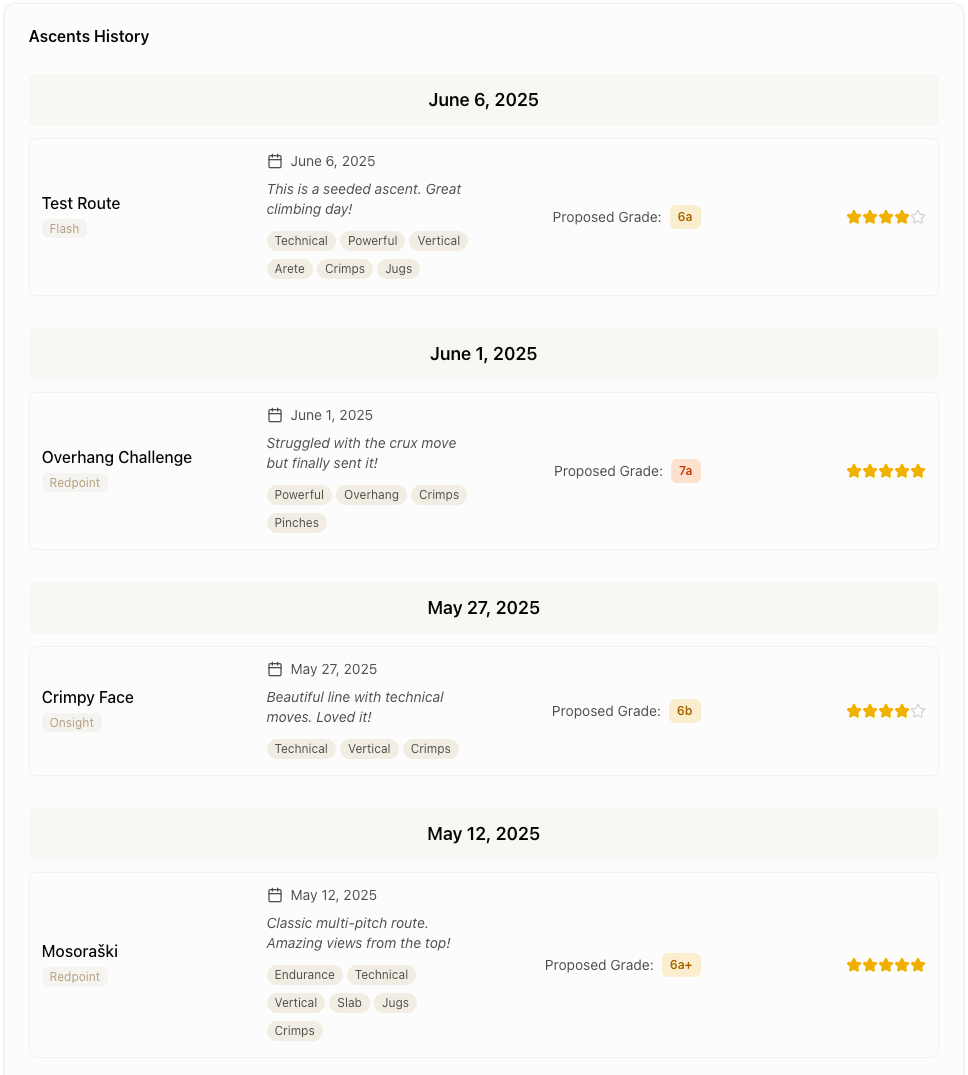
\includegraphics[width=\textwidth]{images/implementacija/web/user-profile-3.png}
        \caption{Web aplikacija}
        \label{fig:korisnicki_profil_povijest_web}
    \end{subfigure}
    \caption{Povijest uspona}
    \label{fig:korisnički_profil_3}
\end{figure}

Osim statistike, profil sadrži i povijest svih uspona, kronološki poredanih od najnovijeg prema najstarijem (slika~\ref{fig:korisnički_profil_3}). Svaki unos u povijest sadrži sve relevantne informacije poput datuma, naziva penjačkog smjera, lokaciju, težinu, stil uspona, osobni komentar i ocjenu smjera te direktnu poveznicu na detaljni pregled samog penjačkog smjera. Ovaj dnevnik služi kao vrijedan alat za prisjećanje na prethodna penjačka iskustva.

\subsection{Korisnički profil drugog korisnika}

Pretraživanjem korisničkog profila drugog korisnika, korisnik može vidjeti statistike, grafove performansi i povijest uspona drugog korisnika na isti način kao i na vlastitom profilu (slika~\ref{fig:korisnički_profil_other}).


\begin{figure}[H]
    \centering
    \begin{subfigure}[b]{0.33\textwidth}
        \centering
        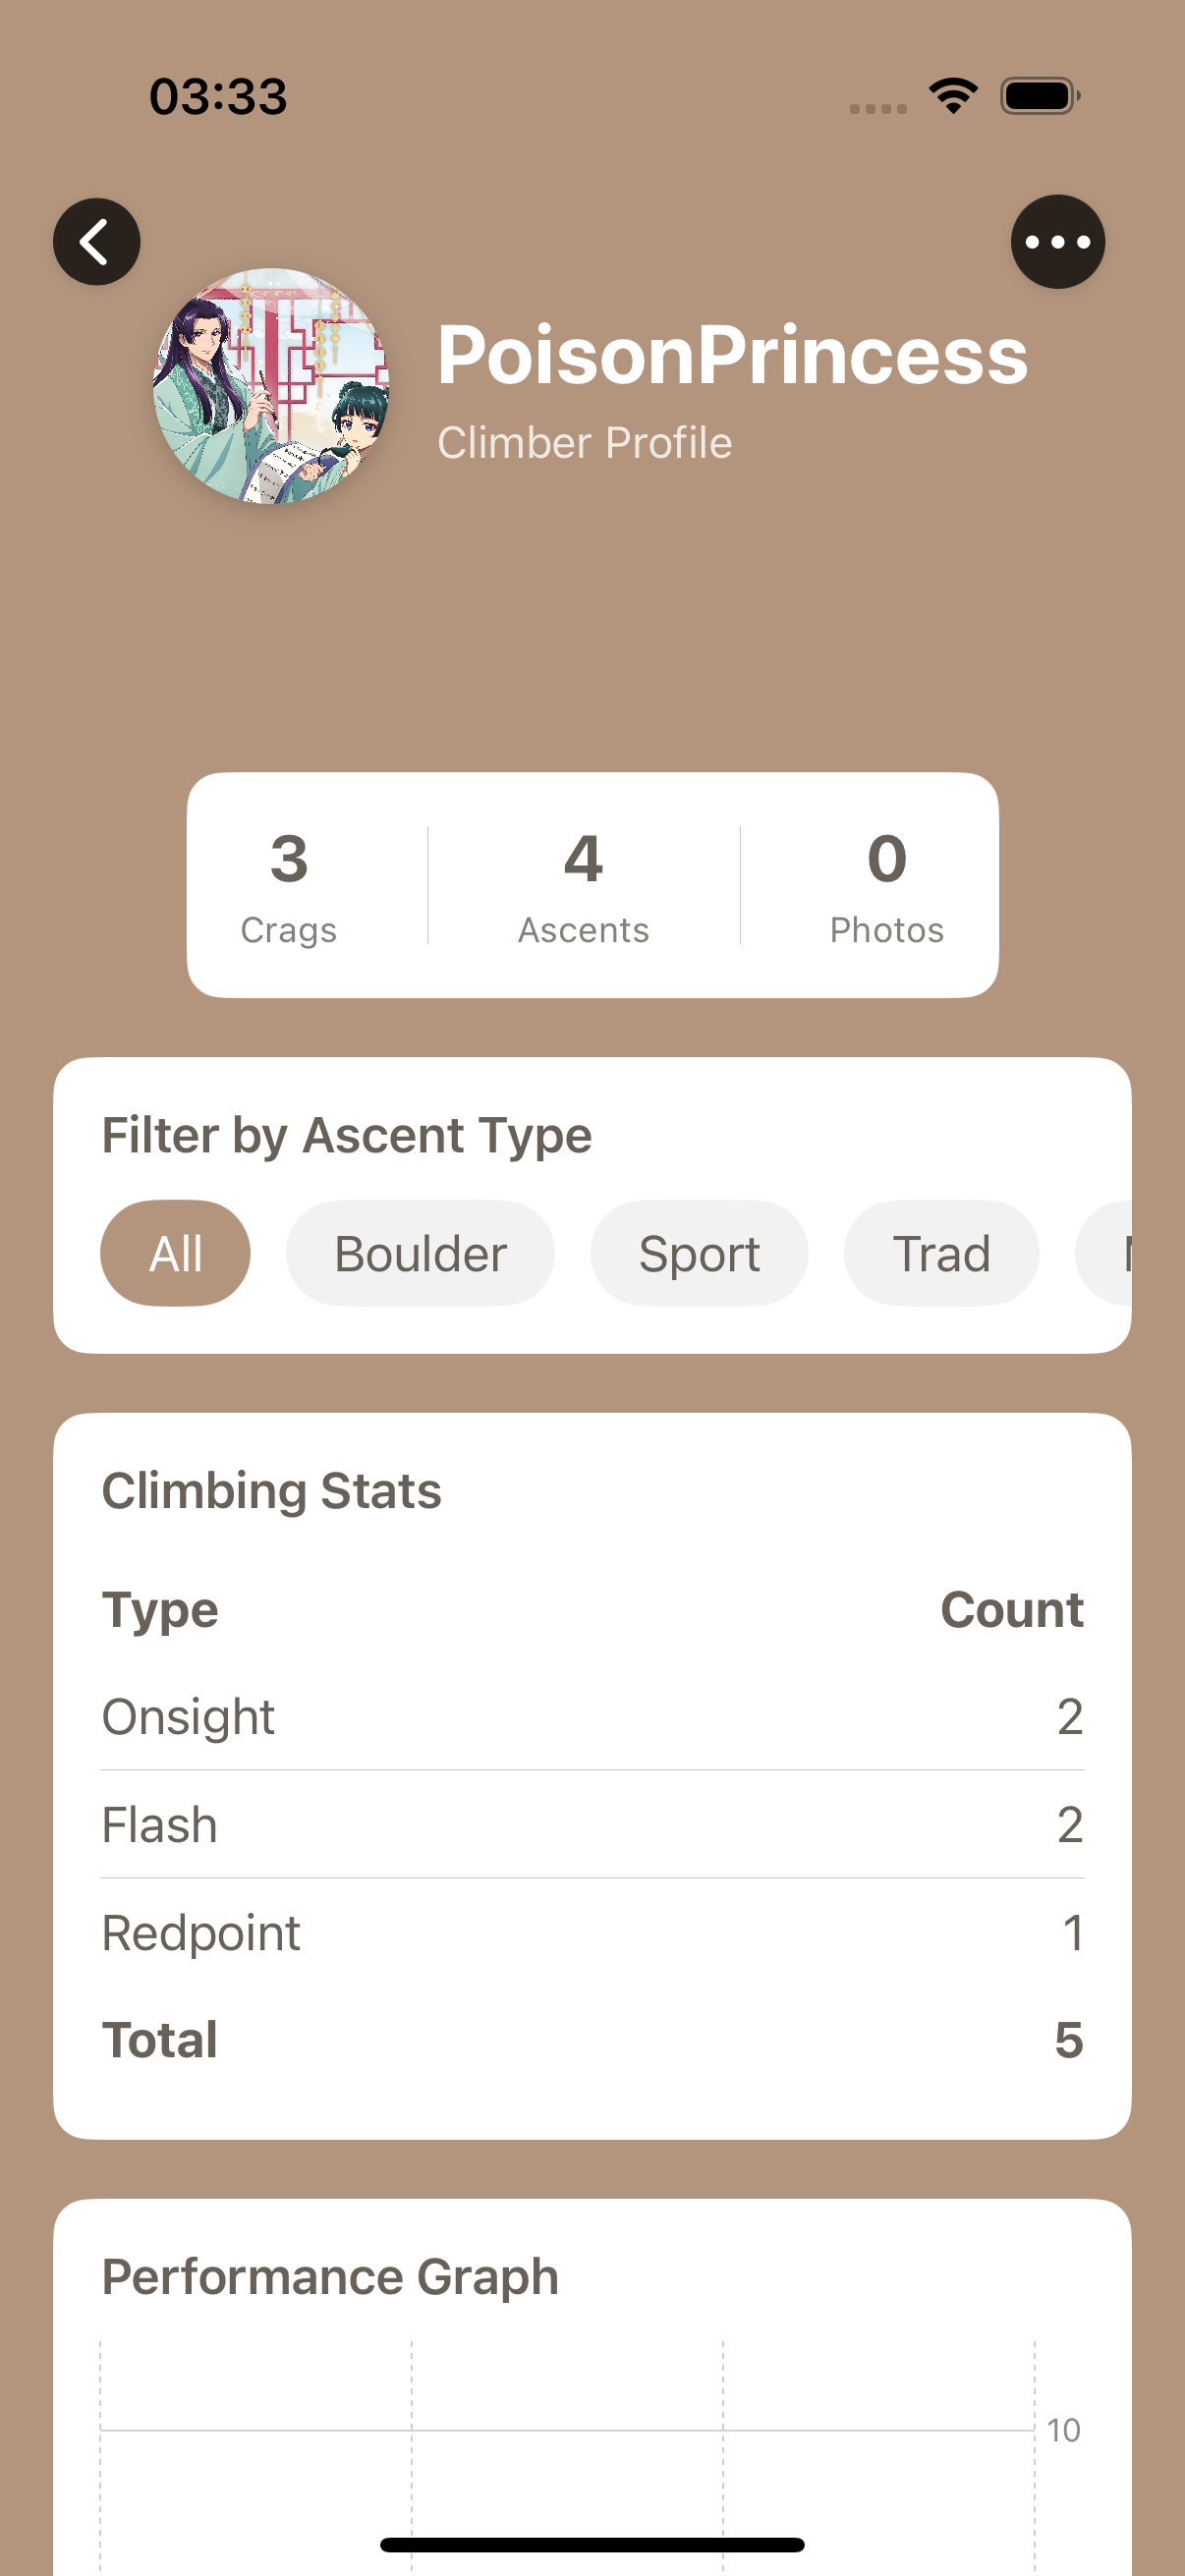
\includegraphics[width=\textwidth]{images/implementacija/user-profile-other.png}
        \caption{Mobilna aplikacija}
        \label{fig:korisnicki_profil_other_mob}
    \end{subfigure}
    \hfill
    \begin{subfigure}[b]{0.65\textwidth}
        \centering
        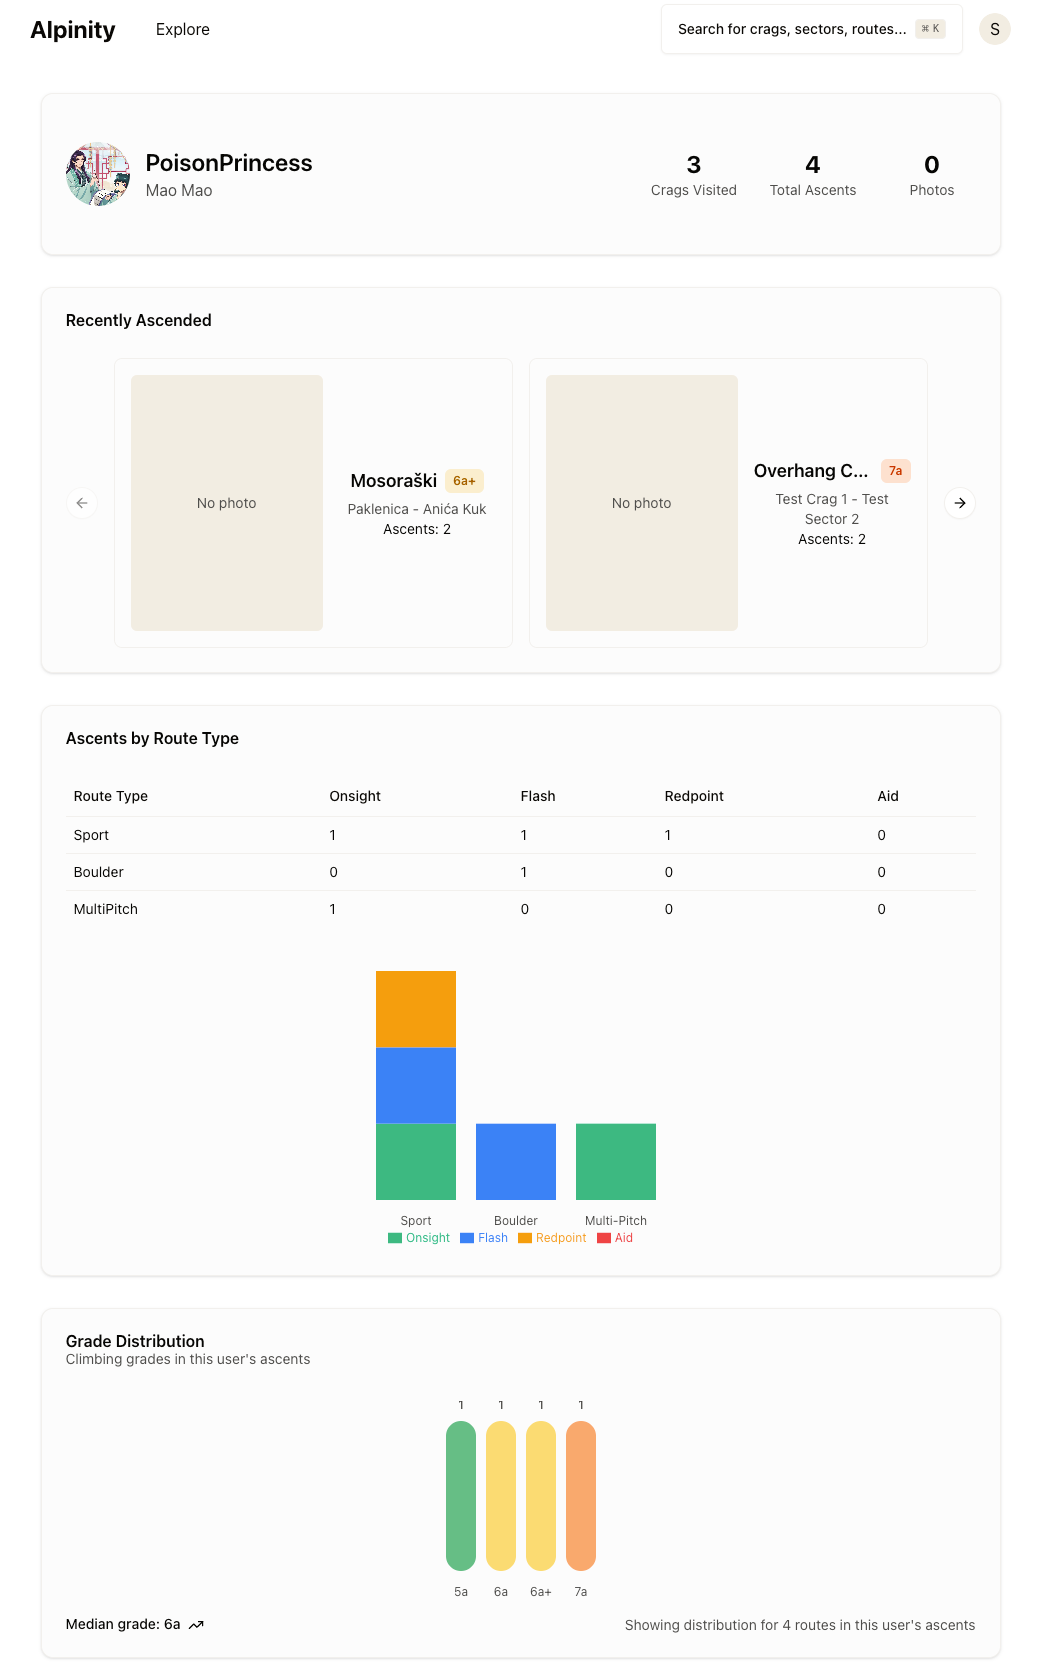
\includegraphics[width=\textwidth]{images/implementacija/web/user-profile-other.png}
        \caption{Web aplikacija}
        \label{fig:korisnicki_profil_other_web}
    \end{subfigure}
    \caption{Korisnički profil drugog korisnika}
    \label{fig:korisnički_profil_other}
\end{figure}
